%%%%%%%%%%%%%%%%%%%%%%% file template.tex %%%%%%%%%%%%%%%%%%%%%%%%%
%
% This is a general template file for the LaTeX package SVJour3
% for Springer journals.          Springer Heidelberg 2010/09/16
%
% Copy it to a new file with a new name and use it as the basis
% for your article. Delete % signs as needed.
%
% This template includes a few options for different layouts and
% content for various journals. Please consult a previous issue of
% your journal as needed.
%
%%%%%%%%%%%%%%%%%%%%%%%%%%%%%%%%%%%%%%%%%%%%%%%%%%%%%%%%%%%%%%%%%%%
%
% First comes an example EPS file -- just ignore it and
% proceed on the \documentclass line
% your LaTeX will extract the file if required
\begin{filecontents*}{example.eps}
%!PS-Adobe-3.0 EPSF-3.0
%%BoundingBox: 19 19 221 221
%%CreationDate: Mon Sep 29 1997
%%Creator: programmed by hand (JK)
%%EndComments
gsave
newpath
  20 20 moveto
  20 220 lineto
  220 220 lineto
  220 20 lineto
closepath
2 setlinewidth
gsave
  .4 setgray fill
grestore
stroke
grestore
\end{filecontents*}
%
\RequirePackage{fix-cm}
%
%\documentclass{svjour3}                     % onecolumn (standard format)
%\documentclass[smallcondensed]{svjour3}     % onecolumn (ditto)
\documentclass[smallextended]{svjour3}       % onecolumn (second format)
%\documentclass[twocolumn]{svjour3}          % twocolumn
%
\smartqed  % flush right qed marks, e.g. at end of proof
%
\usepackage{graphicx}
%
% \usepackage{mathptmx}      % use Times fonts if available on your TeX system
%
% insert here the call for the packages your document requires
%\usepackage{latexsym}
% etc.
%
% please place your own definitions here and don't use \def but
% \newcommand{}{}



% Insert the name of "your journal" with
\journalname{Journal of Computer-Aided Molecular Design}
\begin{document}

\title{Blind prediction of cyclohexane-water distribution coefficients from the SAMPL5 challenge}
\titlerunning{SAMPL5 distribution coefficients}
\thanks{We appreciate financial support from the National Institutes of Health (1R01GM108889-01) and the National Science Foundation (CHE 1352608), and computing support from the UCI GreenPlanet cluster, supported in part by NSF Grant CHE-0840513. 
This work was made possible in part by NIH grant U01 GM111528. The contents of this paper are solely the responsibility of the authors and do not necessarily represent the o?cial views of the NIH.
M.K.G. has an equity interest in and is a cofounder and scienti�c advisor of VeraChem LLC. } % Is this where this belongs?

% CCB: I'm not seeing where the thanks prints. I double checked the JCAMD template and I didn't delete anything
%template example:
%\thanks{Grants or other notes
%about the article that should go on the front page should be
%placed here. General acknowledgments should be placed at the end of the article.}

\author{Caitlin C Bannan         \and
        Kalistyn H Burley \and
        Michael Chiu \and
        Michael K Gilson \and
        David L Mobley
}
% I only included contact info for David, I assume you are the corresponding author and that we only need to include contact info for one person
% The example had the same contact info for all the authors, but we all have different departments/institutions
\institute{C. C. Bannan \at Department of Chemistry, University of California, Irvine
	\and
	K. H. Burley \at Department of Pharmaceutical Sciences, University of California, Irvine
	\and
	M. Chiu \at % institution?
	\and
	M. K. Gilson \at University of California, San Diego % Check department
	\and
	D. L. Mobley \at Department of Chemistry and Department of Pharmaceutical Sciences, University of California, Irvine\\
		147 Bison Modular, Irvine, CA 92697
              Tel.: +949-824-6383\\
              Fax: +949-824-2949\\
              \email{dmobley@mobleylab.org} }          

\date{Received: date / Accepted: date}
% The correct dates will be entered by the editor
\maketitle

\begin{abstract}
% Outline for abstract:
describe DC part of SAMPL5 challenge

We analyze submissions and provide reference calculations

Results, range of RMSE or AUE? Better or worse than expected from past sample challenges?

Conclusions: tautomeric enumeration,  

\keywords{distribution coefficient \and blind challenge \and free energy } 
% CCB: these were options provided by the template, I don't know what they're for.
% \PACS{}
% \subclass{}
\end{abstract}


% ======================================================================================================
% Actual writing starts HERE
% I've tried to remove your comments (that I addressed) and any I was using to help with outlining. Any left over comments should indicate questions or things I know I need to add (such as citations I haven't found yet). 

\section{Introduction}
\label{intro}

This year's Statistical Assessment of Modeling of Proteins and Ligand (SAMPL) challenge focuses on prediction of cyclohexane-water distribution coefficients. 
This focus on distribution coefficients replaces the focus on hydration free energies which has been a fixture of the past five challenges (SAMPL0-4) \cite{Mobley:2014gu,Geballe:2012fc,Geballe:2010jr,Klimovich:2010jm,Mobley:2009iu,Mobley:2012jwa,Nicholls:2008cx}.
Due to a lack of ongoing experimental work, hydration free energies are no longer a practical property for blind challenges. 
It has become increasingly difficult to find unpublished or obscure hydration free energies and therefore impossible to design a challenge focusing on particular compounds, functional groups or chemical classes. 
The past SAMPL challenges have driven real improvements in a variety of methods for calculating hydration free energy \cite{Mobley:2014gu}, so we sought to include a similar physical property in SAMPL5. 
The organizers settled on cyclohexane-water distribution coefficients, and thanks to a partnership with Genetech, were able to conduct a series of measurements on drug-like compounds, discussed in detail in this issue %ref Bas' paper
Measurement is also straightforward enough that future distribution coefficient challenges can be deliberately designed to focus on issues that merit attention to move the field forward.

Partition and distribution coefficients are important physical properties which can provide a valuable opportunity for testing computational methods and molecular models. % cite one of the experimental review papers
Distribution coefficients describe how all forms of a solute distributes itself across two immiscible solvents. 
In this case,
\begin{equation}
D = \frac{\sum_i [X_i]_{cyc}}{\sum_i [X_i]_{aq}}
\label{deflogD}
\end{equation}
where $X_i$ represents a single tautomeric state in one of the solvents and results are reported as the logarithm of this ratio ($\log D$). % probably should cite something here
These are more complicated than partition coefficients ($\log P$), which are limited to a single, typically neutral tautomer \cite{Leo:1971wu}.
$\log P$ is proportional to the transfer free energy, which can be calculated from solvation free energies. % cite all the computational logP papers. 
All tautomers will need to be included to accurately calculate $\log D$, introducing some new complexities avoided in previous hydration free energy studies in SAMPL. 
Accurate tautomer enumeration in both solvents will be an important part of predicting $\log D$. 

% I still can't find any obvious logP or logD challenges, I'll do more googling, but I'm leaving that paragraph out for now. 

Here we discuss results for the SAMPL5 challenge, highlighting difficulties that were common among submissions.
We perform a number of error analyses to determine the best methods.
We also include details for a set of reference calculations we performed estimating $\log D$ as the cyclohexane/water partition coefficient as well as a series of follow-up studies focusing on the importance of tautomers in estimating $\log D$.  
Overall, we believe the outcome of the present SAMPL5 challenge highlights the potential benefits of this type of experimental data to improve computational methods, force fields, sampling algorithms, and treatment of protonation states and tautomers.
Many of these issues will be highly relevant for nominally more challenging problems, such as predictions of protein-ligand binding affinities. 

% I feel like D3R should have come up in the intro... I'm not sure where though. I'm put this here as a reminder to change the first occurrence to their full name. 
% Drug Design Data Resource (D3R)

\section{Challenge Logistics}
\label{logistics}
SAMPL5 began on September 15, 2015
when the specifications for the challenge became available on the D3R website (http://drugdesigndata.org), these are also provided in the supporting information.  
The challenge deadline was February 1, 2016  % I think it technically got extended, but this is the date that is still on the website, should I include the "new" deadline?
and experimental results were provided to participants not long after. 
As in past SAMPL challenges, each group could submit multiple sets of predictions.
There was also the option to remain anonymous.  
A total of 76 prediction sets from 18 participants or participating groups were submitted and assigned a 2 digit ID number 01 to 76 that will be used throughout this paper. 
Predictions were analyzed and overview statistics, as well as individual analysis of each submission by various error metrics (as detailed below) were returned to each participant. 
The challenge culminated with discussions of participants experiences and results at the 1st Annual D3R Workshop at the University of California, San Diego March 9-11, 2016.

% CCB: I thought it made more sense to have the table of molecules earlier, that way we can refer to it and it gives the diversity of molecules when people are reading about the challenge in general. 
\label{results:4}
\begin{table}
\begin{tabular}{|c c c c c c c|}
\hline 
\multicolumn{7}{|c|}{{\small\textbf{Batch 0}}}\\ 
{\scriptsize 003: $ 1.7 \pm 0.2 $ } & {\scriptsize 015: $ 8.8 \pm 1.4 $ } & {\scriptsize 017: $ 3.0 \pm 0.3 $ } & {\scriptsize 020: $ 3.9 \pm 0.4 $ } & {\scriptsize 037: $ 7.5 \pm 1.3 $ } & {\scriptsize 045: $ 1.4 \pm 0.2 $ } & {\scriptsize 055: $ 2.7 \pm 0.2 $ } \\ 
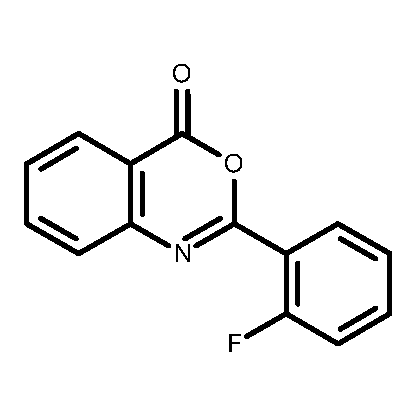
\includegraphics[width = 0.14\textwidth]{2DImages/SAMPL5_003.pdf} & 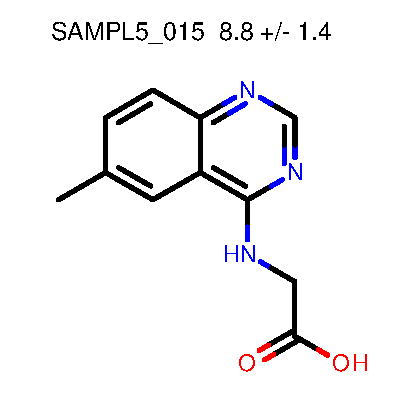
\includegraphics[width = 0.14\textwidth]{2DImages/SAMPL5_015.pdf} & 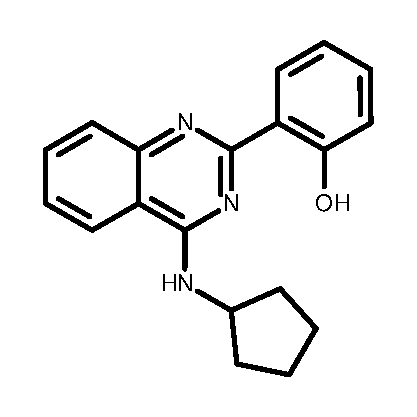
\includegraphics[width = 0.14\textwidth]{2DImages/SAMPL5_017.pdf} & 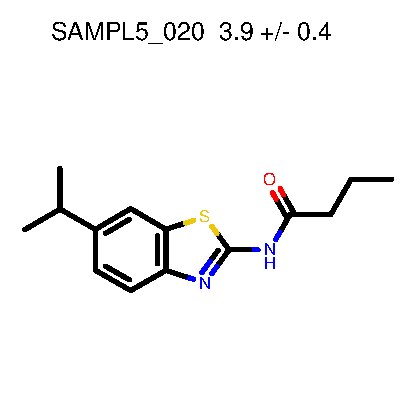
\includegraphics[width = 0.14\textwidth]{2DImages/SAMPL5_020.pdf} & 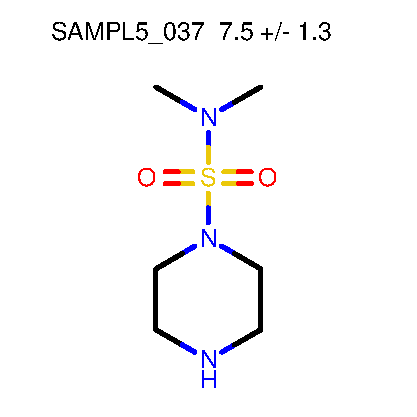
\includegraphics[width = 0.14\textwidth]{2DImages/SAMPL5_037.pdf} & 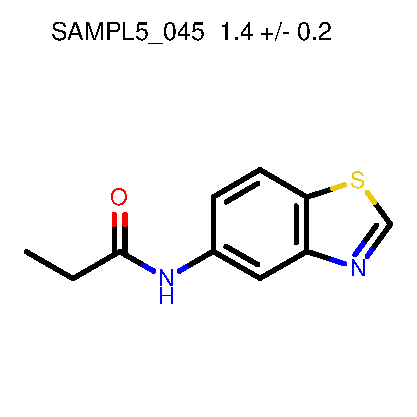
\includegraphics[width = 0.14\textwidth]{2DImages/SAMPL5_045.pdf} & 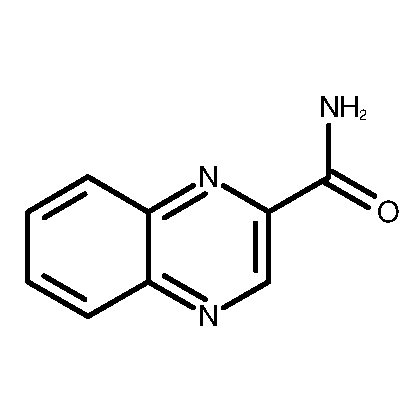
\includegraphics[width = 0.14\textwidth]{2DImages/SAMPL5_055.pdf} \\ 
{\scriptsize 058: $ 2.2 \pm 0.3 $ } & {\scriptsize 059: $ 1.8 \pm 0.2 $ } & {\scriptsize 061: $ 5.9 \pm 1.0 $ } & {\scriptsize 068: $ 2.7 \pm 0.3 $ } & {\scriptsize 070: $ 5.9 \pm 0.8 $ } & {\scriptsize 080: $ 2.6 \pm 0.2 $ } & \\ 
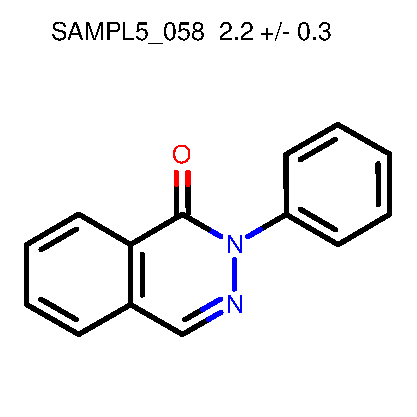
\includegraphics[width = 0.14\textwidth]{2DImages/SAMPL5_058.pdf} & 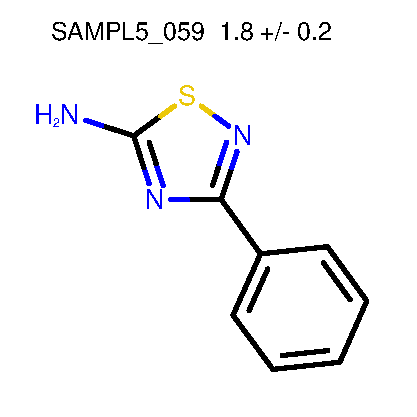
\includegraphics[width = 0.14\textwidth]{2DImages/SAMPL5_059.pdf} & 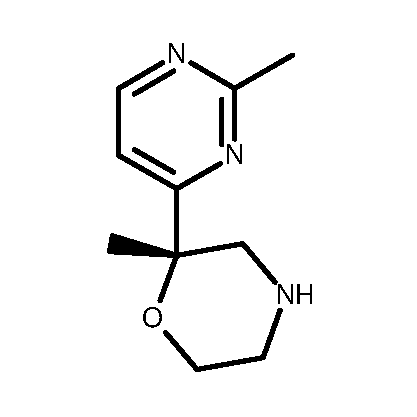
\includegraphics[width = 0.14\textwidth]{2DImages/SAMPL5_061.pdf} & 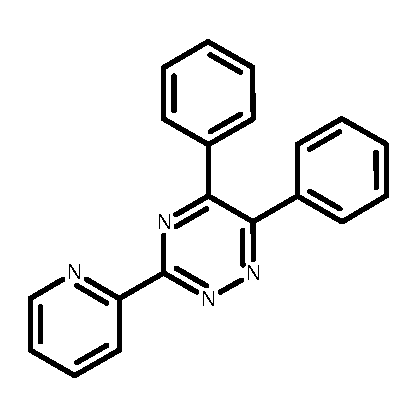
\includegraphics[width = 0.14\textwidth]{2DImages/SAMPL5_068.pdf} & 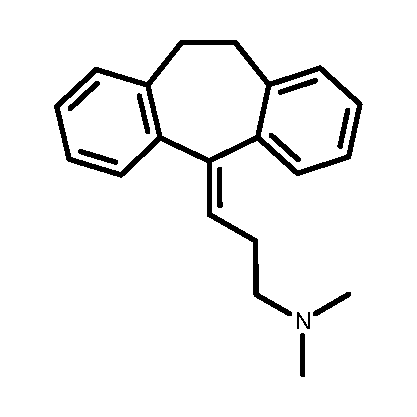
\includegraphics[width = 0.14\textwidth]{2DImages/SAMPL5_070.pdf} & 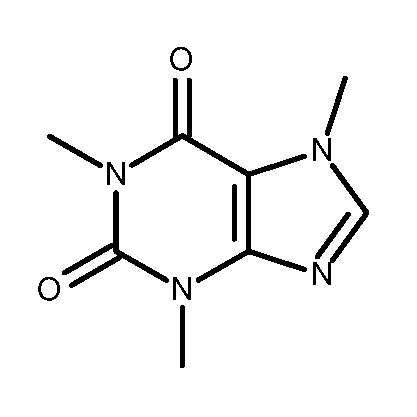
\includegraphics[width = 0.14\textwidth]{2DImages/SAMPL5_080.pdf} & \\ 
\hline 
\multicolumn{7}{|c|}{{\small\textbf{Batch 1}}}\\ 
{\scriptsize 004: $ 2.3 \pm 0.3 $ } & {\scriptsize 005: $ 2.6 \pm 0.3 $ } & {\scriptsize 007: $ 3.1 \pm 0.4 $ } & {\scriptsize 010: $ 7.8 \pm 1.6 $ } & {\scriptsize 011: $ 7.1 \pm 1.3 $ } & {\scriptsize 021: $ 2.2 \pm 0.2 $ } & {\scriptsize 026: $ 8.0 \pm 1.7 $ } \\ 
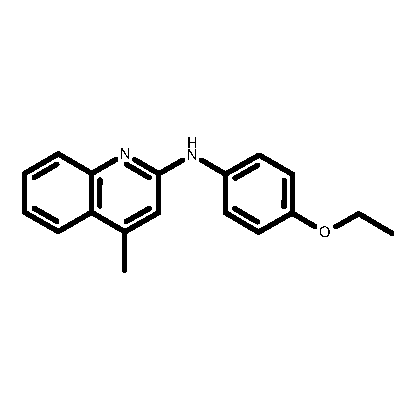
\includegraphics[width = 0.14\textwidth]{2DImages/SAMPL5_004.pdf} & 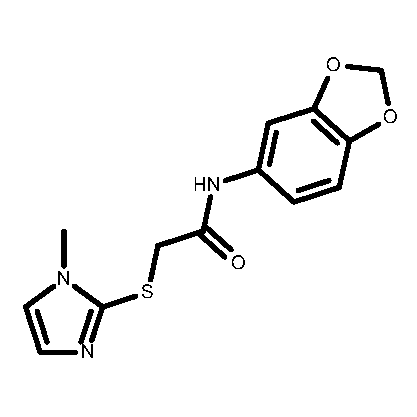
\includegraphics[width = 0.14\textwidth]{2DImages/SAMPL5_005.pdf} & 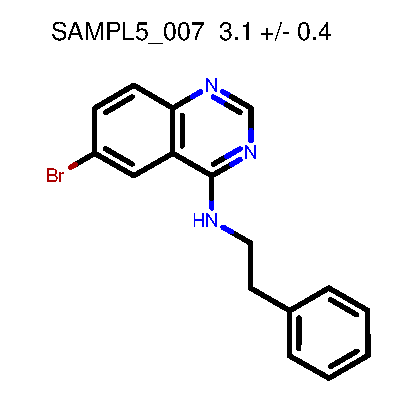
\includegraphics[width = 0.14\textwidth]{2DImages/SAMPL5_007.pdf} & 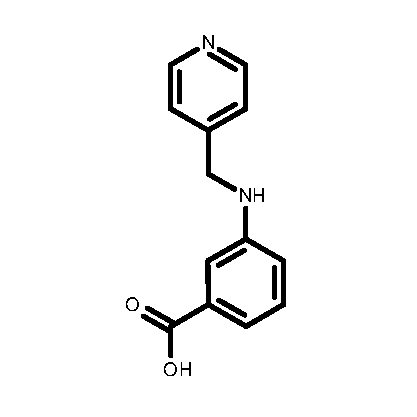
\includegraphics[width = 0.14\textwidth]{2DImages/SAMPL5_010.pdf} & 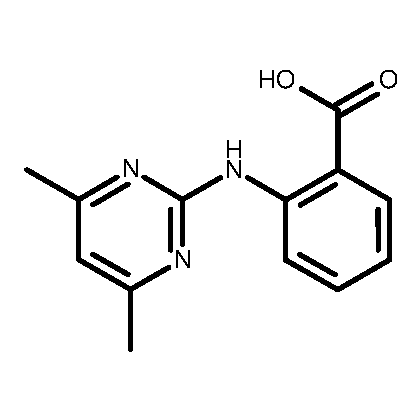
\includegraphics[width = 0.14\textwidth]{2DImages/SAMPL5_011.pdf} & 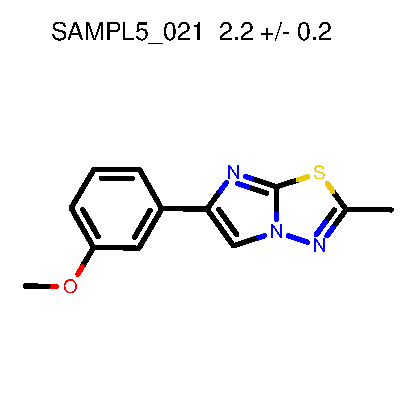
\includegraphics[width = 0.14\textwidth]{2DImages/SAMPL5_021.pdf} & 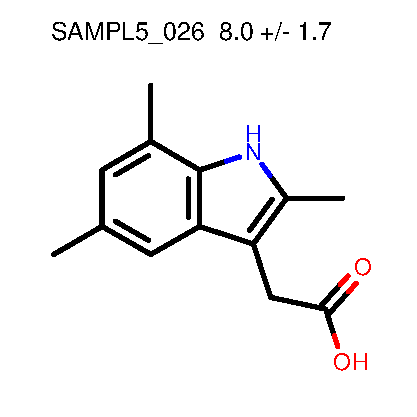
\includegraphics[width = 0.14\textwidth]{2DImages/SAMPL5_026.pdf} \\ 
{\scriptsize 027: $ 3.4 \pm 0.3 $ } & {\scriptsize 042: $ 3.2 \pm 0.4 $ } & {\scriptsize 044: $ 3.7 \pm 0.4 $ } & {\scriptsize 046: $ 2.7 \pm 0.4 $ } & {\scriptsize 047: $ 2.1 \pm 0.3 $ } & {\scriptsize 048: $ 2.7 \pm 0.3 $ } & {\scriptsize 056: $ 3.5 \pm 0.3 $ } \\ 
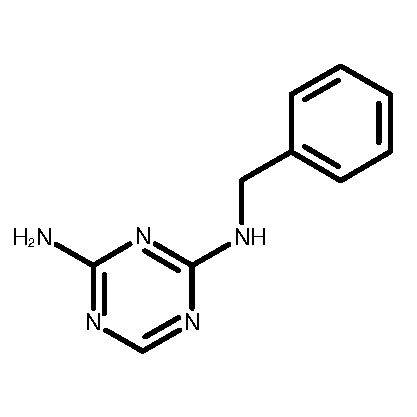
\includegraphics[width = 0.14\textwidth]{2DImages/SAMPL5_027.pdf} & 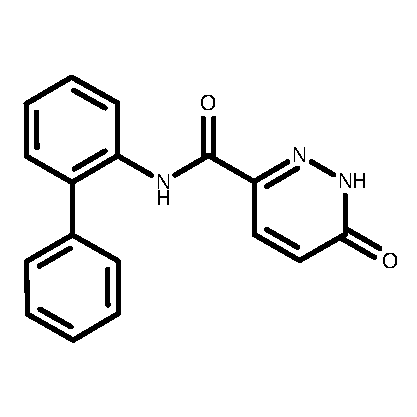
\includegraphics[width = 0.14\textwidth]{2DImages/SAMPL5_042.pdf} & 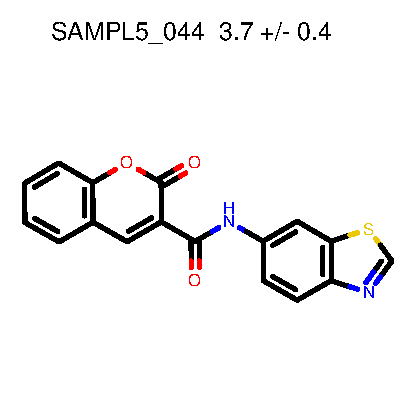
\includegraphics[width = 0.14\textwidth]{2DImages/SAMPL5_044.pdf} & 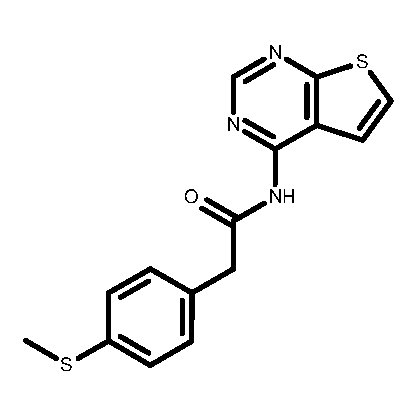
\includegraphics[width = 0.14\textwidth]{2DImages/SAMPL5_046.pdf} & 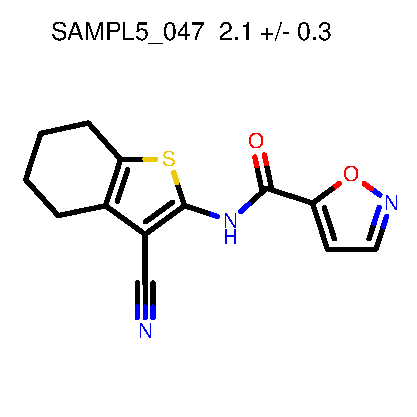
\includegraphics[width = 0.14\textwidth]{2DImages/SAMPL5_047.pdf} & 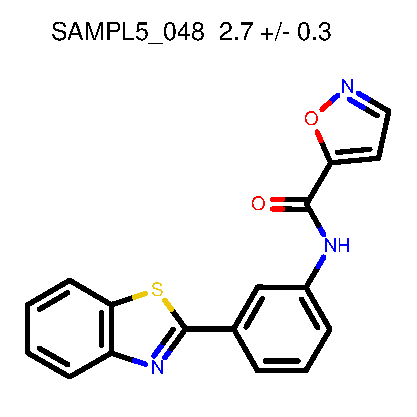
\includegraphics[width = 0.14\textwidth]{2DImages/SAMPL5_048.pdf} & 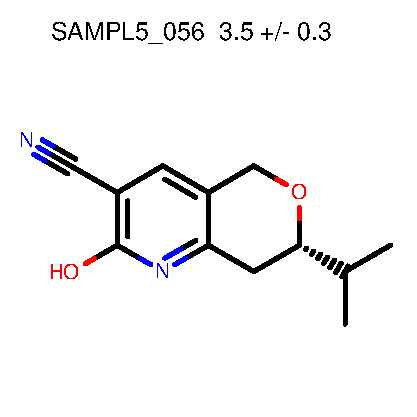
\includegraphics[width = 0.14\textwidth]{2DImages/SAMPL5_056.pdf} \\ 
{\scriptsize 060: $ 6.7 \pm 1.6 $ } & {\scriptsize 063: $ 6.7 \pm 1.0 $ } & {\scriptsize 071: $ 2.8 \pm 0.3 $ } & {\scriptsize 072: $ 4.9 \pm 0.7 $ } & {\scriptsize 081: $ 6.0 \pm 0.8 $ } & {\scriptsize 090: $ 2.8 \pm 0.3 $ } & \\ 
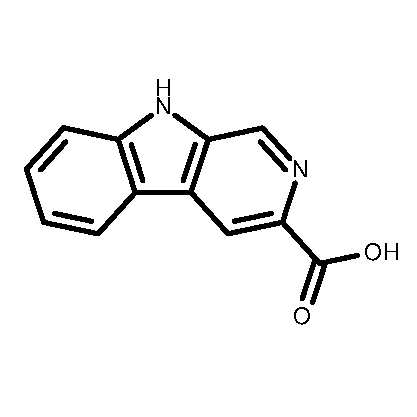
\includegraphics[width = 0.14\textwidth]{2DImages/SAMPL5_060.pdf} & 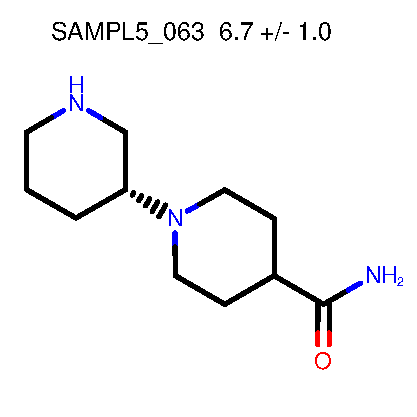
\includegraphics[width = 0.14\textwidth]{2DImages/SAMPL5_063.pdf} & 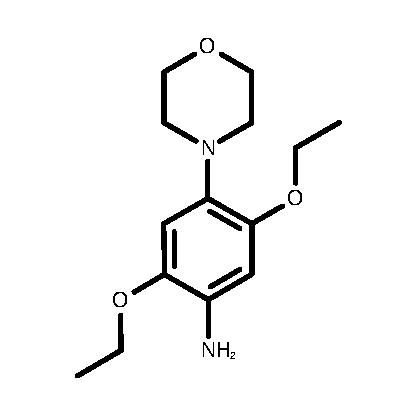
\includegraphics[width = 0.14\textwidth]{2DImages/SAMPL5_071.pdf} & 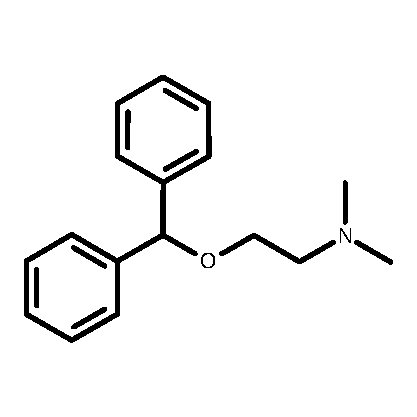
\includegraphics[width = 0.14\textwidth]{2DImages/SAMPL5_072.pdf} & 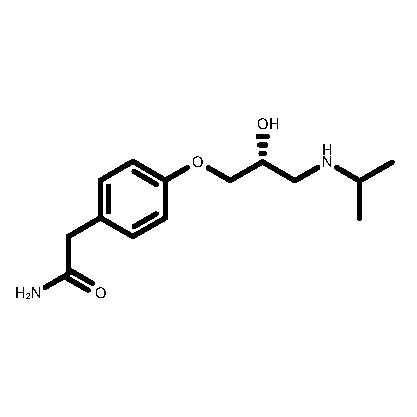
\includegraphics[width = 0.14\textwidth]{2DImages/SAMPL5_081.pdf} & 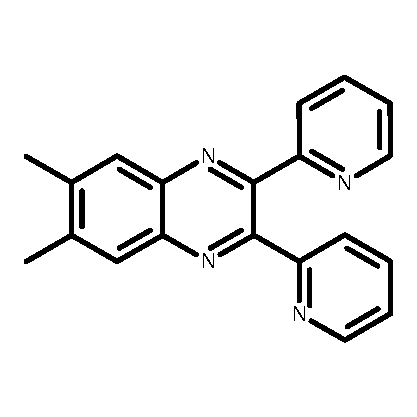
\includegraphics[width = 0.14\textwidth]{2DImages/SAMPL5_090.pdf} & \\ 
\hline 
\multicolumn{7}{|c|}{{\small\textbf{Batch 2}}}\\ 
{\scriptsize 002: $ 2.5 \pm 0.2 $ } & {\scriptsize 006: $ 2.7 \pm 0.4 $ } & {\scriptsize 013: $ 3.1 \pm 0.3 $ } & {\scriptsize 019: $ 3.1 \pm 0.4 $ } & {\scriptsize 024: $ 3.0 \pm 0.4 $ } & {\scriptsize 033: $ 3.0 \pm 0.3 $ } & {\scriptsize 049: $ 2.1 \pm 0.2 $ } \\ 
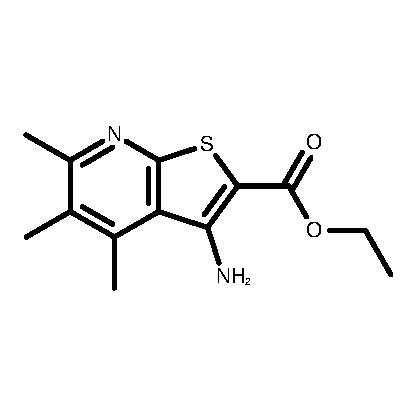
\includegraphics[width = 0.14\textwidth]{2DImages/SAMPL5_002.pdf} & 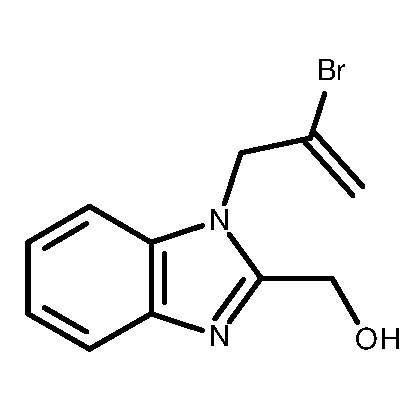
\includegraphics[width = 0.14\textwidth]{2DImages/SAMPL5_006.pdf} & 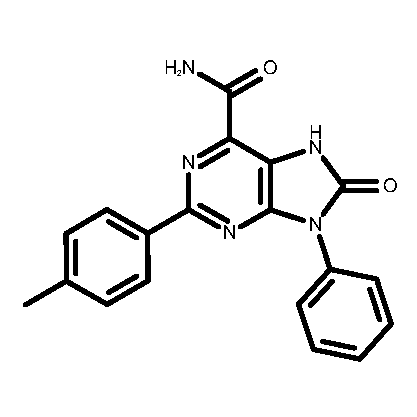
\includegraphics[width = 0.14\textwidth]{2DImages/SAMPL5_013.pdf} & 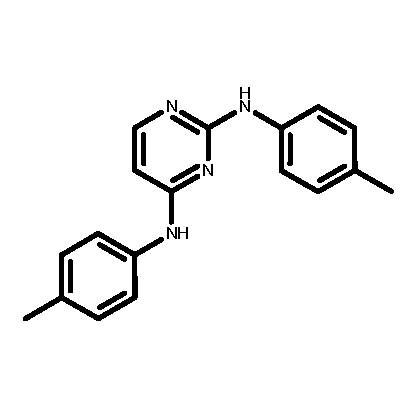
\includegraphics[width = 0.14\textwidth]{2DImages/SAMPL5_019.pdf} & 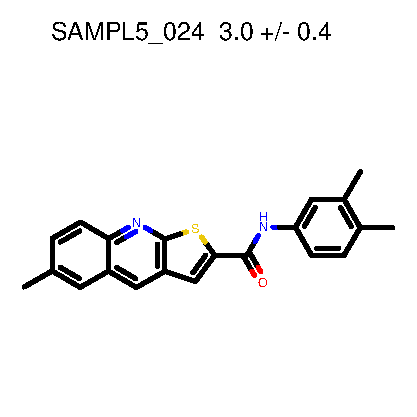
\includegraphics[width = 0.14\textwidth]{2DImages/SAMPL5_024.pdf} & 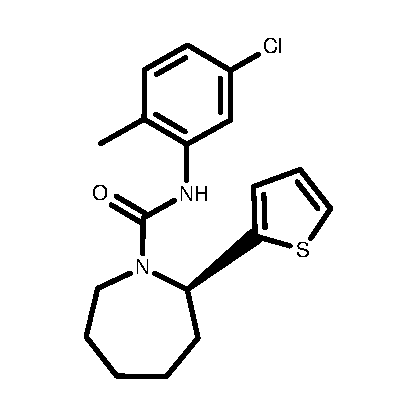
\includegraphics[width = 0.14\textwidth]{2DImages/SAMPL5_033.pdf} & 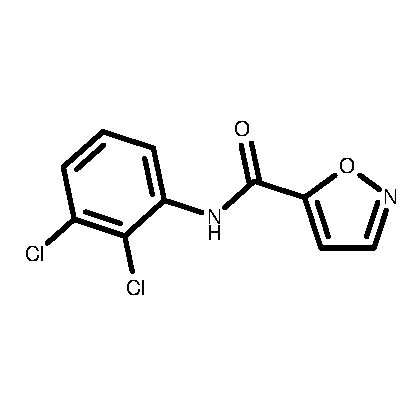
\includegraphics[width = 0.14\textwidth]{2DImages/SAMPL5_049.pdf} \\ 
{\scriptsize 050: $ 5.6 \pm 0.4 $ } & {\scriptsize 065: $ 5.3 \pm 0.5 $ } & {\scriptsize 067: $ 4.5 \pm 0.6 $ } & {\scriptsize 069: $ 3.9 \pm 0.5 $ } & {\scriptsize 074: $ 6.6 \pm 0.4 $ } & {\scriptsize 075: $ 4.8 \pm 0.6 $ } & {\scriptsize 082: $ 5.1 \pm 0.6 $ } \\ 
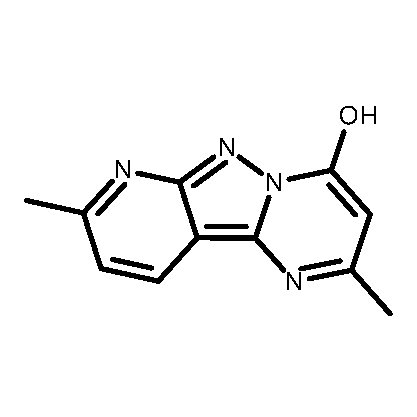
\includegraphics[width = 0.14\textwidth]{2DImages/SAMPL5_050.pdf} & 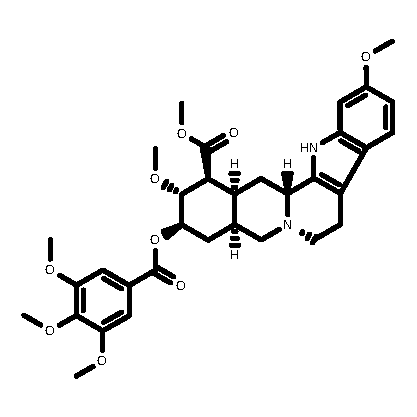
\includegraphics[width = 0.14\textwidth]{2DImages/SAMPL5_065.pdf} & 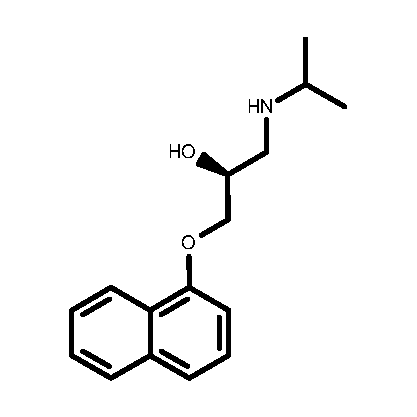
\includegraphics[width = 0.14\textwidth]{2DImages/SAMPL5_067.pdf} & 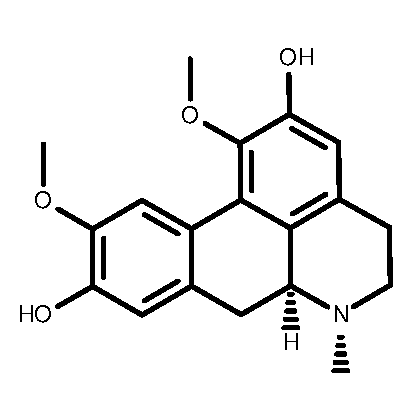
\includegraphics[width = 0.14\textwidth]{2DImages/SAMPL5_069.pdf} & 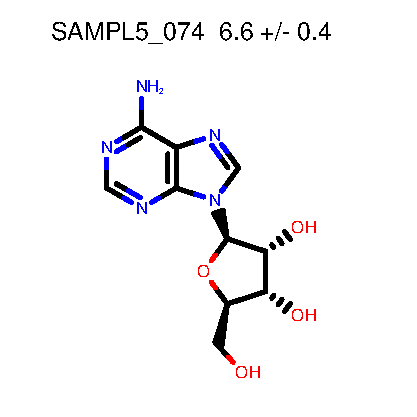
\includegraphics[width = 0.14\textwidth]{2DImages/SAMPL5_074.pdf} & 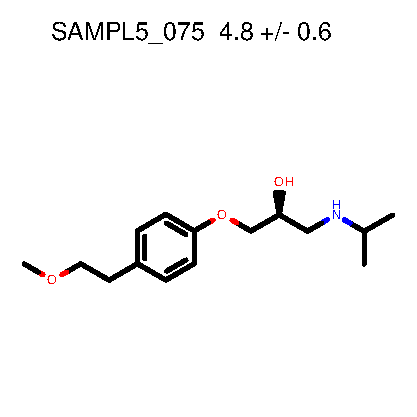
\includegraphics[width = 0.14\textwidth]{2DImages/SAMPL5_075.pdf} & 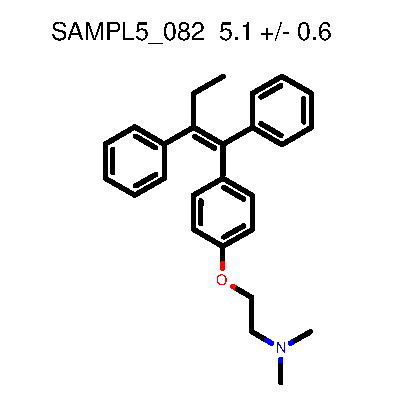
\includegraphics[width = 0.14\textwidth]{2DImages/SAMPL5_082.pdf} \\ 
{\scriptsize 083: $ 8.4 \pm 0.7 $ } & {\scriptsize 084: $ 3.6 \pm 0.5 $ } & {\scriptsize 085: $ 2.8 \pm 0.3 $ } & {\scriptsize 086: $ 4.5 \pm 0.6 $ } & {\scriptsize 088: $ 2.9 \pm 0.4 $ } & {\scriptsize 092: $ 3.9 \pm 0.4 $ } & \\ 
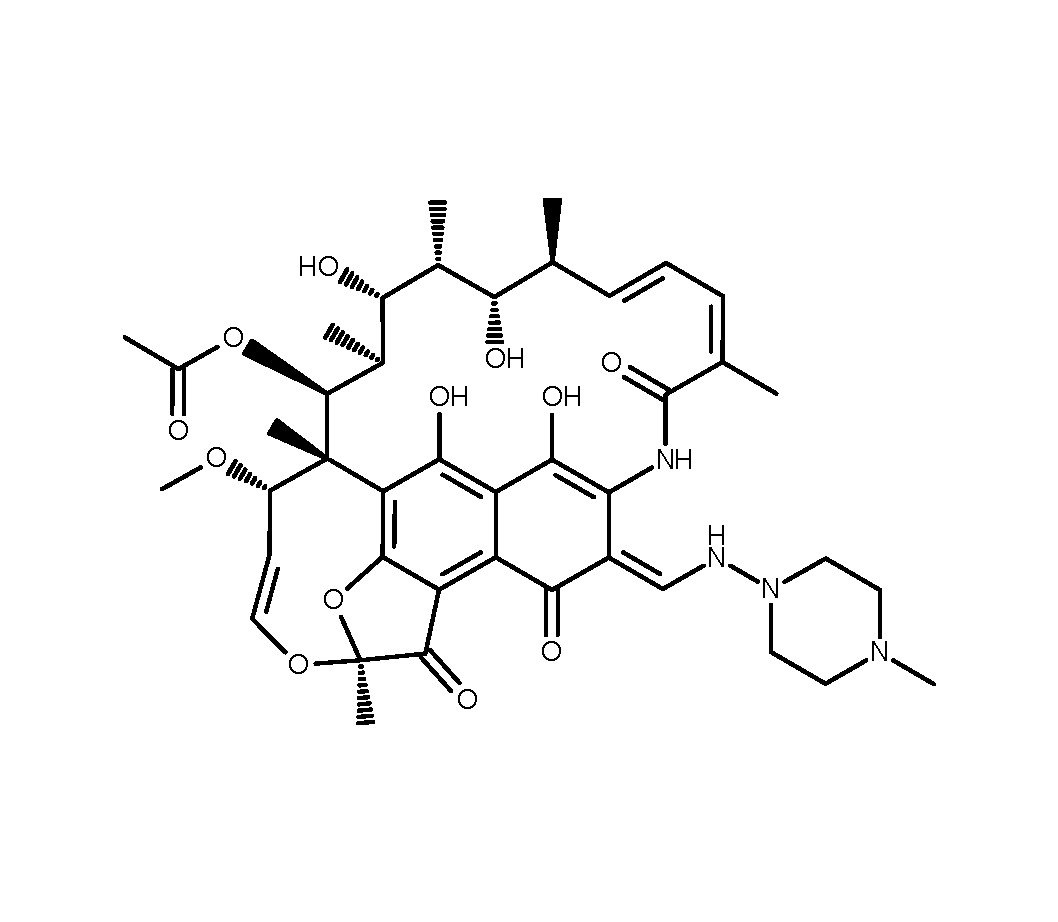
\includegraphics[width = 0.14\textwidth]{2DImages/SAMPL5_083.pdf} & 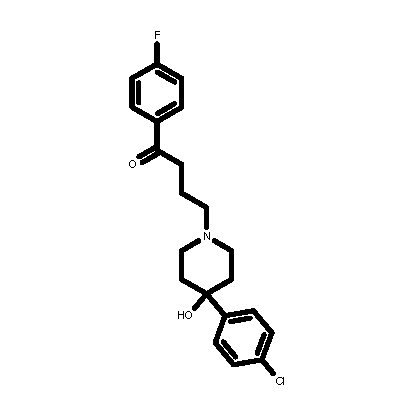
\includegraphics[width = 0.14\textwidth]{2DImages/SAMPL5_084.pdf} & 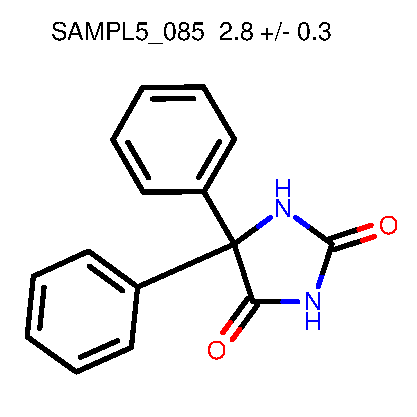
\includegraphics[width = 0.14\textwidth]{2DImages/SAMPL5_085.pdf} & \includegraphics[width = 0.14\textwidth]{2DImages/SAMPL5_086.pdf} & \includegraphics[width = 0.14\textwidth]{2DImages/SAMPL5_088.pdf} & \includegraphics[width = 0.14\textwidth]{2DImages/SAMPL5_092.pdf} & \\ 
\hline
\end{tabular}

\label{MoleculeTable}
\caption{A complete list of compounds used in the SAMPL5, sorted by batch. The average unsigned error, reported in log units, was calculated with all predictions for that compound.} 
\end{table}

For the prediction of distribution coefficients in SAMPL5, a total of 53 molecules were considered. 
Molecules were assigned an identifier in the form SAMPL5\_XXX; the complete table can be found below and in the supporting information. 
The 53 molecules were divided into batches 0, 1, and 2 containing 13, 20, and 20 molecules respectively. 
We wanted each batch to have a similar dynamic range and for the molecules to increase in size, so on average the smallest molecules are in batch 0 and the largest in batch 2. 
To control for dynamic range, molecules were grouped by calculated octanol/water partition coefficient and then by molecular weight. 
The smallest molecules from each partition coefficient group were added to batch 0, then batch 1, the rest of the molecules compromise batch 2.

Participants could submit just batch 0, batches 0 and 1, or batches 0, 1, and 2. 
The idea was that all participants should attempt predictions on the full set if at all possible, but grouping into batches would allow people with particularly demanding methods (such as polarizable force fields or methods requiring intensive quantum mechanics) to focus on smaller compounds and still be evaluated. 
Eight submissions from two participants submitted results for only batch 0, an additional five submissions from two participants provided only batch 0 and batch 1.
Here we focus on the results for the complete set of molecules (batches 0, 1, and 2). 
Separate analysis for the other submission options (batch 0 or batches 0 and 1) is available in the supporting information.
Included in the challenge information was the SMILES string for each molecule as well as mol2 and SDfiles. 
All information provided to challenge participants is included in supporting information. 

Participants were asked to report a cyclohexane/water distribution coefficient for each molecule. 
As discussed above, distribution coefficients are the ratio of concentrations for all forms of the solute in cyclohexane and the aqueous layer. 
During the experimental measurements, the water layer was an aqueous buffer at pH 7.4. 
We also required participants to provide two estimates for uncertainty, a statistical uncertainty for their computational method and a model uncertainty that estimates agreement with experiment.  
The statistical uncertainty should be the variation expected from repeated computational calculations. 
The model uncertainty, on the other hand, is an estimate of how well the calculated value will agree with experiment. 
For example, in a recent study we computed cyclohexane/water partition coefficients using alchemical solvation free energy calculations in GROMACS where the statistical uncertainties were around 0.05
but the root mean squared error was around 1.4 log units. 
An important part of creating predictive models is the ability to know when it will fail. 
Analysis of model uncertainties then, is an important part of evaluating any model. 

\section{Error metrics} % probably need a different section title here.... 
\label{analysisMethods}

Similar to past SAMPL challenges, we considered a large number of error metrics in analyzing all predictions submitted to SAMPL5. 
Each error metric was calculated for all submissions, by batch and distributed to challenge participants before the workshop.
Here we will focus primarily on six error metrics: the root-mean-squared error (RMSE), average unsigned error (AUE), average signed error (ASE), Pearson's R (R), Kendall's tau (tau), and the `error slope' explained in depth below. 
We also calculated maximum absolute error and percent of predictions with the correct sign which are not included in the analysis here, but were provided to challenge participants and available in the supporting information.
Uncertainty in each metric was calculated as the standard deviation in 1000 bootstrap trials. 
As described previously, this bootstrapping technique included variation in the experimental values based on their reported uncertainties\cite{Mobley:2014gu}. % Cite anything else?

As discussed above, an important evaluation of a predictive tool is the ability to estimate how well and when a computational method will agree with experiment. 
As in SAMPL4 \cite{Mobley:2014gu}, a quantile-quantile plot (QQ Plot) was created for each prediction set. % cite stats paper that describes them in depth and  
QQ Plots compare a normal distribution with how well a set of predictions agree with experiment according to the model uncertainty. 
For example, consider the number of predictions within one standard deviation of the expected value, the value on the x-axis represents the normal distribution (0.68) and the value on the y-axis will represent the fraction of predictions that are within one model uncertainty of the experimental value.  % read again with a set of fresh eyes
A regression analysis helps summarize these results.
The `error slope' is the slope of the line comparing the fraction of predictions within range of experiment to the expected fraction in a normal distribution.
An error slope of greater than one indicates that the calculated values are within uncertainty of experiment more often than expected, or in other words the model uncertainty was over estimated. 
Oppositely, an error slope less than one suggests the model uncertainty was underestimated. 

The last goal of prediction analysis was to identify any individual molecules where most of the methods failed to accurately estimate the distribution coefficient. 
To accomplish this a data set was created for each molecule consisting of all predictions submitted for that molecule, then all the error metrics discussed above were calculated for each molecule. 
Here we will primarily focus on just average unsigned error for molecules, but all other error metrics were provided to participants and available in supporting information. 

\section{Reference calculations from the Mobley group} 
\label{methods:1}

We calculated distribution coefficients through a few different methods as a reference. 
KHB, a graduate student in the Mobley group, performed a set of blind calculations estimating the $\log D$ as a partition coefficient between cyclohexane and water calculated from solvation free energies.
In addition, CCB and DLM performed calculations after the challenge which were not included with the prediction sets. 
We considered a null hypothesis where all molecules are assumed to distribute equally between cyclohexane and water.
Many fast structural based tools for octanol/water partition coefficients exist, which we compared with no and little correction for cyclohexane. 
We also included post challenge analysis of protonation and tautomeric states as a correction from calculated partition coefficients to distribution coefficients

\subsection{Calculating partition coefficients from solvation free energies}
\label{methods:2}
% Can you (and how would you) cite a paper that is still in review? I've written this assuming we can point to my logP paper, but it's not actually available yet. 
Partition coefficients are the ratio of concentrations of a solute in a single tautomeric state distributed between two solvents. 
Before the challenge, each molecule was taken directly as the provided SMILES string with no further tautomer enumeration.
As demonstrated in the literature, % cite previous logP from free energy in logP paper, mine?
partition coefficients are directly proportional to the difference between the solvation free energy for the solute into each solvent. 
We use previously established and automated protocols %logP paper, 
to calculate the solvation free energy of each molecule into water and cyclohexane. 
Then the calculated partition coefficient was reported as an estimate for $\log D$. 

To calculate solvation free energies, we used automated tools created by the Mobley lab.
Molecular dynamics simulations were performed in GROMACS  \cite{Berendsen:1995gro,Hess:2008db,Lindahl:2001gro3,vanderSpoel:2005hz,Pronk:2013ef,Pall:2014gb,Abraham:2015gj}
with the General AMBER Force Field (GAFF) \cite{Wang:2004dev} with AM1-BCC charges\cite{Jakalian:2000ki,Jakalian:2002bd}.
Topology and coordinate files for the solvated boxes with 1 solute molecule and 500 cyclohexane or 1000 water molecules were built using the Solvation Toolkit. % cite logP paper
These files were then converted to AMBER, DESMOND, and LAMMPS formats and provided to SAMPL5 participants. % citation for file formats?
The Solvation Toolkit takes advantage of many open source Python modules and is available at https://github.com/MobleyLab/SolvationToolkit.
It converts SMILES strings or IUPAC names of any mixture of compounds to parameterized molecules and builds topology and coordinate files for a variety of simulation packages. 
All molecular dynamics parameters are identical to previous studies \cite{Liu:2016kb,Klimovich:2010jm}. % add logP paper
The molecule is taken from the solvated box to a non-interacting gas phase in 20 lambda values. 
Solvation free energies are calculated with Alchemical Analysis tool \cite{Klimovich:2015er}
using the multi-state Bennett acceptance ratio to extract free energy difference between the beginning and end state. 
The partition coefficient was calculated as the difference between the cyclohexane solvation free energy and the hydration free energy.
The statistical uncertainty was reported as the propagated uncertainty from the solvation free energy calculations. 
The model uncertainty was estimated to be the same for all molecules and reported as the root-mean-squared error from a recent study on calculating cyclohexane/water partition coefficient, specifically 1.4 log units. % cite logP paper
These were assigned submission ID 39 and included in the error analysis performed on all submissions.

\paragraph{Simulation box size does not affect the calculated solvation free energy.} 
Hydration free energies were previously shown to be independent of box sizes from 2 to 9 nanometers, within calculated uncertainties \cite{Parameswaran:2014kq}. 
% are there calculations where box size effects the results? Should we be citing a paper related to that?
Polar solutes are more likely to significantly affect long range interactions so we calculated the dipole moment of each SAMPL5 molecule using the position and charges on atoms in the mol2 files. 
SAMPL5\_024 had the largest dipole moment so it was used as the solute for the box size investigation. 
The solvation free energy calculations were set up as described above, changing the number of cyclohexane molecules from 100 to 500.  
% I'm still not completely clear on how using reaction field affects the calculation, I know they change the way coulomb interactions are calculated at a longer distance?
Our calculations above are performed with pme coulomb interactions, here we also repeated the solvation free energy calculations with reaction field coulomb interactions assigning the dielectric coefficient for cyclohexane, 2.043 \cite{crc}.
\begin{figure} 
\includegraphics{boxSize.eps}
\caption{This is a figure for the box size study}
\label{boxSizes}  
\end{figure}
We found that for 2.5 to 4.5 nm box edges there is no significant change in the calculated solvation free energy for SAMPL5\_024 in cyclohexane. % fill in reaction field differences... 
The input, results, molecular dynamics parameter files, and tables of solvation free energies are available in the supporting information. 

\subsection{Consideration of tautomers after SAMPL5}
\label{methods:3}

To help understand the results from our partition coefficient calculations could have been improved, we considered corrections for changes in the solutes protonation or tautomeric states.  
Distribution coefficients different from partition coefficients in that they include all forms of the solute in both solvents. 
A common way to correct between experimentally measured distribution coefficients and partition coefficients is with pKa values for the solute. 
This is a simple correction using the Henderson-Hasselbalch 
equation:
\begin{equation}
pH = pK_a + \log \frac{X}{HX}
\label{HH}
\end{equation}
to relate the concentration of neutral species to the charged species at a given pH. 
This correction will depend on if the neutral solute is acidic or basic. 
The equation used to calculate a distribution coefficient ($\log D$) from a partition coefficient ($\log P$) for a basic solute (or X in eqn. \ref{HH}) is below  
\begin{equation}
\log D = \log P - log(1+10^{pK_a-pH})
\label{basic}
\end{equation}
Alternatively for an acid solute (or HX in eqn. \ref{HH}) we would instead use:
\begin{equation}
\log D = \log P - log(1+10^{pH-pK_a})
\label{acidic}
\end{equation}
We use Schr\"{o}dinger's Epik tool % citations
to calculate pKa values for each molecule according to experimental conditions. 
We then estimated a $\log D$ using the equations above. 
Using pKa values only accounts for one change in protonation, whereas a correct distribution coefficient should include all relevant tautomers and protonation states of the molecule in both solvents. 
To correct for all other tautomer states we used Schr\"{o}dinger's LigPrep % citations
to enumerate tautomers for each molecule in the aqueous solution. 
The results of the enumeration includes a energetic "state penalty" which relates the population of that tautomer to all others. 
This state penalty can be converted into log units and used as a correction term to convert $\log P$ to $\log D$:
\begin{equation}
\log D = \log P + \frac{-E_{state penalty}}{k_BT \ln (10)}
\label{statepenalty}
\end{equation}
where $k_B$ is Boltzmann constant and T is temperature. 
LigPrep can only perform the tautomer enumeration with water or DMSO as a solvent, so we were unable to predict tautomers in cyclohexane. 
Therefor both of these corrections account for the protonation or tautomer states only in the aqueous layer and assume the tautomer remains fixed in cyclohexane as the one used in the initial simulation. 

\subsection{Estimating distribution coefficients with a fast, structural based partition coefficient calculator}
\label{methods:4}
Many structural based tools exist for octanol/water partition coefficients; they are very fast and generally accurate. 
However, these tools are all trained on empirical data, meaning they are limited by the training data. 
We chose the OpenEye tool OEXlogP \cite{RenxiaoWang:1997fa,Wang:2000kk} as an example of such a tool. 
Two post prediction sets were prepared with the OEXlogP tool.
First, the predicted octanol/water partition coefficient was considered an estimate for $\log D$.
In the second set, we calculated a correction for the bias between the calculated XlogP values and a set of experimental cyclohexane/water partition coefficients \cite{Leo:1971wu}.
For the rest of this paper we will refer to the octanol/water partition coefficient set as $XlogP_{oct}$ and the bias corrected set as $XlogP_{corr}$. 

\section{Results and Discussion}
\label{results:1}
% Since there is so much diversity in the better performing methods this is more of a paragraph about the variety of submission. I thought it would be a good way to open results and gives some context. 
% I'm still working on exactly how to group and word this - you should probably skip it on this read. 
Cyclohexane/water distribution coefficients were predicted by a broad range of methods for the SAMPL5 challenge. 
A large portion of predictions used alchemical molecular dynamics simulations to estimate the solvation free energy in explicit solvent using fixed-charge all-atom force fields, all-atom/course-grained hybrid force fields, and polarizing force fields. 
Other methods include 3D-RISM, EC-RISM, COSMO-RS, QM/MM, ... 

SAMPL5 is the first to include distribution coefficients, but we can estimate how well we expect submissions to do based on past SAMPL challenges which included hydration free energies. 
Distribution coefficients can be related to transfer free energy between solvents, which allows us to estimate an expected performance from root-mean-squared errors (RMSE) in past hydration free energy calculations. 
In SAMPL4 \cite{Mobley:2014gu}, the average RMSE for the best half of submissions was about 1.5 kcal/mol which would correspond to 1.54 log units error in a distribution coefficient. 
In contrast, only five submissions had an RMSE less than 2.5 log units. 
 
\begin{table}
\scriptsize
\footnotesize
\begin{tabular}{l l l l l l l}
\hline
ID & Ave. err. & RMS & AUE & tau & R & Err. slope \\ 
\hline
01\textsuperscript{1} & $2.3 \pm 0.8$ & $5.1 \pm 0.5$ & $4.3 \pm 0.5$ & $0.13 \pm 0.12$ & $0.20 \pm 0.17$ & $0.44 \pm 0.09$ \\ 
02 & $-0.5 \pm 0.3$ & $2.3 \pm 0.3$ & $1.7 \pm 0.2$ & $0.48 \pm 0.07$ & $0.63 \pm 0.07$ & $0.69 \pm 0.07$ \\ 
03\textsuperscript{1} & $-7.6 \pm 3.5$ & $21.3 \pm 2.6$ & $15.9 \pm 2.5$ & $0.52 \pm 0.10$ & $0.59 \pm 0.12$ & $-0.00 \pm 0.00$ \\ 
04\textsuperscript{0} & $1.6 \pm 0.5$ & $2.5 \pm 0.6$ & $1.9 \pm 0.4$ & $0.77 \pm 0.12$ & $0.87 \pm 0.05$ & $0.77 \pm 0.12$ \\ 
05 & $-8.2 \pm 0.4$ & $8.7 \pm 0.5$ & $8.2 \pm 0.4$ & $0.29 \pm 0.09$ & $0.39 \pm 0.11$ & $0.21 \pm 0.03$ \\ 
06 & $1.8 \pm 0.5$ & $4.0 \pm 0.3$ & $3.4 \pm 0.3$ & $0.46 \pm 0.09$ & $0.61 \pm 0.10$ & $0.58 \pm 0.07$ \\ 
07 & $0.5 \pm 0.4$ & $3.3 \pm 0.4$ & $2.5 \pm 0.3$ & $0.34 \pm 0.08$ & $0.51 \pm 0.11$ & $0.33 \pm 0.07$ \\ 
08 & $-1.7 \pm 0.4$ & $3.5 \pm 0.5$ & $2.5 \pm 0.3$ & $0.58 \pm 0.06$ & $0.70 \pm 0.06$ & $0.60 \pm 0.08$ \\ 
09 & $6.5 \pm 0.6$ & $7.8 \pm 0.6$ & $6.5 \pm 0.6$ & $-0.29 \pm 0.08$ & $-0.40 \pm 0.10$ & $0.35 \pm 0.07$ \\ 
10 & $0.3 \pm 0.4$ & $3.1 \pm 0.3$ & $2.6 \pm 0.3$ & $0.51 \pm 0.07$ & $0.69 \pm 0.07$ & $0.79 \pm 0.07$ \\ 
11 & $-4.4 \pm 1.8$ & $13.3 \pm 2.6$ & $6.9 \pm 1.6$ & $0.45 \pm 0.09$ & $0.53 \pm 0.09$ & $0.39 \pm 0.08$ \\ 
12 & $-5.5 \pm 2.5$ & $19.4 \pm 1.8$ & $15.0 \pm 1.6$ & $0.37 \pm 0.09$ & $0.39 \pm 0.12$ & $-0.00 \pm 0.00$ \\ 
13\textsuperscript{0} & $-11.1 \pm 5.0$ & $21.0 \pm 4.9$ & $12.2 \pm 4.8$ & $0.56 \pm 0.16$ & $0.43 \pm 0.22$ & $0.59 \pm 0.17$ \\ 
14 & $-0.7 \pm 0.3$ & $2.7 \pm 0.4$ & $2.0 \pm 0.3$ & $0.57 \pm 0.06$ & $0.72 \pm 0.06$ & $0.66 \pm 0.08$ \\ 
15 & $-1.4 \pm 0.4$ & $3.3 \pm 0.5$ & $2.3 \pm 0.3$ & $0.57 \pm 0.07$ & $0.70 \pm 0.06$ & $0.61 \pm 0.07$ \\ 
16 & $0.5 \pm 0.3$ & $2.1 \pm 0.2$ & $1.7 \pm 0.2$ & $0.73 \pm 0.04$ & $0.84 \pm 0.04$ & $0.46 \pm 0.08$ \\ 
17 & $-4.2 \pm 0.4$ & $5.0 \pm 0.4$ & $4.2 \pm 0.4$ & $0.36 \pm 0.08$ & $0.51 \pm 0.10$ & $0.50 \pm 0.07$ \\ 
18 & $-0.8 \pm 0.4$ & $2.7 \pm 0.4$ & $2.0 \pm 0.3$ & $0.47 \pm 0.07$ & $0.60 \pm 0.08$ & $0.62 \pm 0.08$ \\ 
19 & $1.5 \pm 0.3$ & $2.7 \pm 0.2$ & $2.3 \pm 0.2$ & $0.54 \pm 0.07$ & $0.75 \pm 0.07$ & $0.83 \pm 0.06$ \\ 
20 & $-2.3 \pm 0.4$ & $3.6 \pm 0.5$ & $2.7 \pm 0.3$ & $0.55 \pm 0.07$ & $0.70 \pm 0.06$ & $0.48 \pm 0.08$ \\ 
21 & $-1.2 \pm 0.5$ & $3.4 \pm 0.7$ & $2.4 \pm 0.3$ & $0.44 \pm 0.08$ & $0.45 \pm 0.16$ & $0.58 \pm 0.08$ \\ 
22 & $1.6 \pm 0.5$ & $3.9 \pm 0.3$ & $3.1 \pm 0.3$ & $0.29 \pm 0.09$ & $0.48 \pm 0.11$ & $0.68 \pm 0.08$ \\ 
23 & $1.9 \pm 0.5$ & $4.0 \pm 0.4$ & $3.0 \pm 0.4$ & $0.42 \pm 0.07$ & $0.58 \pm 0.08$ & $0.78 \pm 0.08$ \\ 
24\textsuperscript{0} & $2.3 \pm 0.7$ & $3.3 \pm 0.8$ & $2.5 \pm 0.6$ & $0.77 \pm 0.13$ & $0.88 \pm 0.05$ & $0.67 \pm 0.15$ \\ 
25 & $0.0 \pm 0.5$ & $3.6 \pm 0.3$ & $2.9 \pm 0.3$ & $0.53 \pm 0.07$ & $0.70 \pm 0.07$ & $0.71 \pm 0.07$ \\ 
26 & $2.3 \pm 0.7$ & $5.6 \pm 0.4$ & $4.6 \pm 0.4$ & $0.25 \pm 0.08$ & $0.37 \pm 0.11$ & $0.46 \pm 0.07$ \\ 
27 & $-0.2 \pm 0.4$ & $2.6 \pm 0.4$ & $1.8 \pm 0.2$ & $0.49 \pm 0.07$ & $0.61 \pm 0.08$ & $0.66 \pm 0.08$ \\ 
28 & $-2.3 \pm 0.4$ & $3.6 \pm 0.4$ & $2.7 \pm 0.3$ & $0.54 \pm 0.07$ & $0.69 \pm 0.06$ & $0.47 \pm 0.07$ \\ 
29 & $-6.7 \pm 0.4$ & $7.2 \pm 0.4$ & $6.7 \pm 0.4$ & $0.33 \pm 0.08$ & $0.45 \pm 0.11$ & $0.28 \pm 0.04$ \\ 
30 & $2.5 \pm 0.5$ & $4.3 \pm 0.3$ & $3.7 \pm 0.3$ & $0.39 \pm 0.10$ & $0.52 \pm 0.11$ & $0.53 \pm 0.07$ \\ 
31 & $-1.0 \pm 0.3$ & $2.7 \pm 0.3$ & $2.0 \pm 0.3$ & $0.56 \pm 0.07$ & $0.72 \pm 0.06$ & $0.63 \pm 0.08$ \\ 
32 & $2.5 \pm 0.4$ & $3.5 \pm 0.3$ & $3.1 \pm 0.2$ & $0.47 \pm 0.06$ & $0.64 \pm 0.07$ & $0.25 \pm 0.06$ \\ 
33 & $-0.1 \pm 0.5$ & $3.4 \pm 0.3$ & $2.8 \pm 0.3$ & $0.53 \pm 0.08$ & $0.71 \pm 0.08$ & $0.73 \pm 0.07$ \\ 
34 & $-1.3 \pm 0.4$ & $3.0 \pm 0.4$ & $2.2 \pm 0.3$ & $0.56 \pm 0.06$ & $0.69 \pm 0.07$ & $0.61 \pm 0.08$ \\ 
35 & $0.5 \pm 0.4$ & $2.9 \pm 0.3$ & $2.2 \pm 0.2$ & $0.36 \pm 0.08$ & $0.54 \pm 0.10$ & $0.35 \pm 0.07$ \\ 
36 & $1.1 \pm 0.3$ & $2.6 \pm 0.2$ & $2.1 \pm 0.2$ & $0.57 \pm 0.06$ & $0.75 \pm 0.06$ & $0.50 \pm 0.07$ \\ 
37\textsuperscript{0} & $-7.1 \pm 5.1$ & $19.6 \pm 4.3$ & $13.9 \pm 3.9$ & $0.59 \pm 0.16$ & $0.41 \pm 0.22$ & $-0.00 \pm 0.00$ \\ 
38 & $0.8 \pm 0.4$ & $3.3 \pm 0.3$ & $2.7 \pm 0.3$ & $0.41 \pm 0.08$ & $0.58 \pm 0.08$ & $0.78 \pm 0.07$ \\ 
39 & $1.6 \pm 0.3$ & $2.6 \pm 0.2$ & $2.1 \pm 0.2$ & $0.49 \pm 0.08$ & $0.65 \pm 0.10$ & $0.63 \pm 0.08$ \\ 
40 & $0.4 \pm 0.4$ & $2.6 \pm 0.3$ & $1.9 \pm 0.2$ & $0.48 \pm 0.08$ & $0.61 \pm 0.08$ & $1.16 \pm 0.05$ \\ 
41 & $0.3 \pm 0.4$ & $3.2 \pm 0.3$ & $2.7 \pm 0.3$ & $0.53 \pm 0.07$ & $0.69 \pm 0.07$ & $0.77 \pm 0.07$ \\ 
42 & $4.6 \pm 0.4$ & $5.3 \pm 0.4$ & $4.6 \pm 0.4$ & $0.50 \pm 0.08$ & $0.61 \pm 0.12$ & $0.15 \pm 0.05$ \\ 
43 & $-0.7 \pm 0.4$ & $3.0 \pm 0.3$ & $2.3 \pm 0.3$ & $0.51 \pm 0.08$ & $0.67 \pm 0.09$ & $0.94 \pm 0.07$ \\ 
44 & $-0.6 \pm 0.3$ & $2.4 \pm 0.3$ & $1.8 \pm 0.2$ & $0.47 \pm 0.07$ & $0.63 \pm 0.07$ & $0.70 \pm 0.07$ \\ 
45 & $0.9 \pm 0.5$ & $3.6 \pm 0.3$ & $2.9 \pm 0.3$ & $0.38 \pm 0.08$ & $0.58 \pm 0.10$ & $0.71 \pm 0.07$ \\ 
46 & $-8.3 \pm 0.5$ & $9.1 \pm 0.6$ & $8.3 \pm 0.5$ & $0.23 \pm 0.08$ & $0.31 \pm 0.10$ & $0.14 \pm 0.03$ \\ 
47 & $-1.3 \pm 0.4$ & $3.3 \pm 0.5$ & $2.2 \pm 0.3$ & $0.58 \pm 0.07$ & $0.71 \pm 0.06$ & $0.62 \pm 0.08$ \\ 
48 & $1.5 \pm 0.4$ & $3.0 \pm 0.3$ & $2.3 \pm 0.3$ & $0.38 \pm 0.07$ & $0.55 \pm 0.08$ & $0.42 \pm 0.07$ \\ 
49 & $-1.1 \pm 0.4$ & $3.3 \pm 0.4$ & $2.6 \pm 0.3$ & $0.42 \pm 0.07$ & $0.58 \pm 0.07$ & $0.78 \pm 0.07$ \\ 
50\textsuperscript{1} & $-7.1 \pm 2.5$ & $16.6 \pm 3.0$ & $9.2 \pm 2.3$ & $0.60 \pm 0.08$ & $0.66 \pm 0.08$ & $0.38 \pm 0.09$ \\ 
51 & $1.7 \pm 0.7$ & $5.2 \pm 0.4$ & $4.3 \pm 0.4$ & $0.31 \pm 0.08$ & $0.46 \pm 0.10$ & $0.46 \pm 0.08$ \\ 
52\textsuperscript{0} & $-3.5 \pm 1.2$ & $5.4 \pm 0.7$ & $4.8 \pm 0.7$ & $0.56 \pm 0.14$ & $0.59 \pm 0.13$ & $0.23 \pm 0.10$ \\ 
53 & $0.5 \pm 0.4$ & $2.8 \pm 0.3$ & $2.2 \pm 0.2$ & $0.44 \pm 0.09$ & $0.58 \pm 0.10$ & $1.00 \pm 0.06$ \\ 
54 & $-1.0 \pm 0.3$ & $2.7 \pm 0.3$ & $1.9 \pm 0.2$ & $0.56 \pm 0.07$ & $0.70 \pm 0.06$ & $0.65 \pm 0.08$ \\ 
55\textsuperscript{1} & $-11.6 \pm 3.4$ & $22.3 \pm 3.1$ & $13.7 \pm 3.1$ & $0.59 \pm 0.09$ & $0.61 \pm 0.12$ & $0.38 \pm 0.09$ \\ 
56 & $-1.1 \pm 0.4$ & $3.3 \pm 0.5$ & $2.2 \pm 0.3$ & $0.57 \pm 0.06$ & $0.71 \pm 0.06$ & $0.67 \pm 0.08$ \\ 
57 & $-10.2 \pm 2.4$ & $20.2 \pm 2.2$ & $12.6 \pm 2.2$ & $0.43 \pm 0.09$ & $0.42 \pm 0.12$ & $0.38 \pm 0.07$ \\ 
58 & $-2.9 \pm 0.5$ & $4.8 \pm 0.5$ & $3.8 \pm 0.4$ & $0.30 \pm 0.10$ & $0.44 \pm 0.12$ & $0.55 \pm 0.08$ \\ 
59\textsuperscript{0} & $-4.2 \pm 1.0$ & $5.6 \pm 0.6$ & $5.2 \pm 0.6$ & $0.54 \pm 0.15$ & $0.55 \pm 0.14$ & $0.13 \pm 0.08$ \\ 
60 & $0.2 \pm 0.4$ & $2.5 \pm 0.4$ & $1.9 \pm 0.2$ & $0.49 \pm 0.08$ & $0.60 \pm 0.08$ & $1.02 \pm 0.06$ \\ 
61 & $-1.2 \pm 0.4$ & $3.4 \pm 0.6$ & $2.4 \pm 0.3$ & $0.44 \pm 0.08$ & $0.45 \pm 0.16$ & $0.53 \pm 0.07$ \\ 
62 & $0.7 \pm 0.5$ & $3.5 \pm 0.4$ & $2.7 \pm 0.3$ & $0.27 \pm 0.09$ & $0.38 \pm 0.12$ & $0.73 \pm 0.07$ \\ 
63 & $-4.5 \pm 1.8$ & $13.3 \pm 2.6$ & $6.9 \pm 1.6$ & $0.45 \pm 0.09$ & $0.52 \pm 0.09$ & $0.41 \pm 0.08$ \\ 
64 & $1.3 \pm 0.7$ & $5.2 \pm 0.4$ & $4.4 \pm 0.4$ & $0.35 \pm 0.08$ & $0.51 \pm 0.11$ & $0.43 \pm 0.07$ \\ 
65 & $-2.2 \pm 0.5$ & $4.4 \pm 0.5$ & $3.5 \pm 0.4$ & $0.24 \pm 0.10$ & $0.35 \pm 0.12$ & $0.61 \pm 0.08$ \\ 
66 & $1.4 \pm 0.7$ & $5.4 \pm 0.4$ & $4.6 \pm 0.4$ & $0.34 \pm 0.08$ & $0.51 \pm 0.10$ & $0.41 \pm 0.07$ \\ 
67\textsuperscript{0} & $-5.0 \pm 3.0$ & $11.9 \pm 4.3$ & $6.2 \pm 2.8$ & $0.59 \pm 0.18$ & $0.58 \pm 0.13$ & $0.56 \pm 0.17$ \\ 
68 & $2.5 \pm 0.4$ & $3.6 \pm 0.3$ & $3.1 \pm 0.2$ & $0.47 \pm 0.07$ & $0.64 \pm 0.07$ & $0.25 \pm 0.06$ \\ 
69\textsuperscript{0} & $-5.1 \pm 3.0$ & $11.9 \pm 4.5$ & $6.2 \pm 2.9$ & $0.59 \pm 0.16$ & $0.57 \pm 0.12$ & $0.59 \pm 0.17$ \\ 
70\textsuperscript{1} & $-7.0 \pm 2.7$ & $16.5 \pm 3.2$ & $9.2 \pm 2.4$ & $0.60 \pm 0.09$ & $0.67 \pm 0.08$ & $0.36 \pm 0.09$ \\ 
71 & $-10.7 \pm 0.4$ & $11.2 \pm 0.5$ & $10.7 \pm 0.4$ & $0.22 \pm 0.08$ & $0.29 \pm 0.11$ & $0.16 \pm 0.03$ \\ 
72 & $-2.6 \pm 0.4$ & $4.2 \pm 0.6$ & $3.0 \pm 0.4$ & $0.56 \pm 0.06$ & $0.70 \pm 0.06$ & $0.45 \pm 0.07$ \\ 
73 & $0.3 \pm 0.3$ & $2.4 \pm 0.3$ & $1.8 \pm 0.2$ & $0.48 \pm 0.08$ & $0.64 \pm 0.08$ & $0.50 \pm 0.08$ \\ 
74 & $-2.7 \pm 0.4$ & $4.2 \pm 0.5$ & $3.0 \pm 0.4$ & $0.56 \pm 0.07$ & $0.70 \pm 0.06$ & $0.44 \pm 0.08$ \\ 
75 & $4.1 \pm 0.4$ & $5.1 \pm 0.3$ & $4.4 \pm 0.3$ & $0.23 \pm 0.09$ & $0.34 \pm 0.11$ & $0.29 \pm 0.06$ \\ 
76 & $1.7 \pm 0.7$ & $5.3 \pm 0.4$ & $4.3 \pm 0.4$ & $0.32 \pm 0.08$ & $0.47 \pm 0.11$ & $0.47 \pm 0.08$ \\ 
\hline 
\end{tabular}

\label{groupStats}
\caption{Error metrics were calculate for each set of predictions, including root-mean-squared error (RMSE), average unsigned error (AUE), average signed error (ASE), Kendall's tau (tau), and Pearson's R (R). Error slope refers to the slope of data in a QQ Plot. Indicated submissions only included batch 0\textsuperscript{a} or batches 0 and 1\textsuperscript{b}.} 
\end{table}
%CCB: I right justified, it looks a little better, I had to take it down another font size to fit on one page, but I think if we could put the caption to the side instead of under the table it would fit with one font size up, one of the SAMPL4 tables was like that, we can probably just leave it as is for submission and adjust if we need to later. 

\begin{figure*} % for 2 column use
\includegraphics{ExamplePlots.eps} % I think they want file names (not labels) to be figure numbers, but that might just be if you're using word... I read it somewhere
\caption{These are examples of plots created for each set of predictions. They were chosen to try to represent the average submissions, those that were in the middle by most error metrics. a and b) comparison plots showing how predicted distribution coefficients compared to experiment for both groups. c,d) QQ Plots showing how their actual predictions were distributed compared to expectations given the model uncertainty.}
\label{examplePlots}       
\end{figure*}

As discussed above, we calculated root-mean-squared error (RMSE), average unsigned error (AUE), average signed error (ASE), Pearson's R (R), Kendall's tau (tau), and the slope from the QQ plot (error slope) for each set of predictions.
These are reported for all submissions (Table \ref{groupStats}), but the rest of the analysis will focus only on submissions that reported 
For each group, we also created a plot comparing their predictions to experimental results.
A few example plots are provided (Fig. \ref{examplePlots}) these represent a typical submission, in that these groups were in the middle of the pack by most error metrics. 
Comparison and QQ plots for every submission are available in the supporting information as well as error metric tables broken down by batch. 

\begin{figure*} 
\includegraphics{ErrorMetrics.eps}
\caption{}
\label{histogramsAverage}       
\end{figure*}

\begin{figure*} 
\includegraphics{CorrelationMetrics.eps}
\caption{}
\label{histogramsCorrelations}       
\end{figure*}

% histograms and batches
To help visualize all of the error metrics, the data was compiled into a histogram where results are sorted from best to worst for that metric (closest to 1 for error slope for example). 
These metrics are split into measurements of deviation from experiment (Fig. \ref{histogramsAverage}) and correlation with experiment (Fig. \ref{histogramsCorrelations}) distinctions which helped in identifying high performing groups. 
This analysis included only submissions that included data for all molecules, the other submissions were indicated in Table \ref{groupStats} and generally fall in the middle of the pack on most metrics.
In comparing methods by all of the error metrics, it is important to keep in mind the uncertainty in these error metrics. 
While Figures \ref{histogramsAverage} and \ref{histogramsCorrelations} show the sorted methods, in reality there are many submissions that are not significantly different from one another. 

In considering the results for the error slope analysis, participants generally tend to do poorly estimating model uncertainty. 
The top three submissions are the only within uncertainty of 1.
Andrew Paluch from Miami University used conservative estimates based on results in previous calculations for solubility and hydration free energy for submissions 53 and 60. % cite paper
Gerhard Koenig from Max-Planck-Institut fuer Kohlenforschung provided no explicit discussion of model uncertainty with submission 43. % cite paper if submitting
Only submission 40 significantly overestimated their model uncertainty.
% is it better to say nothing than to say they didn't include a discussion? 
All other submissions have an error slope below one, indicating a significant underestimation of the model uncertainty. 
% maybe one more sentence about improving error calculations. 

\subsection{Top performing submissions} 
\label{results:2}
\begin{figure*} 
\includegraphics{BestGroups.eps}
\caption{}
\label{BestGroups}      
\end{figure*}

In order to determine which submissions performed the best, we will group error metrics into two categories. 
How well the predictions directly agree with experiment (RMSE and AUE) and then how well correlated the predictions are with experiment (tau and R). 
Unlike past SAMPL challenges, there does appear to be one submission which performs the best by all of these metrics, submission 16. 
There are two additional submissions which performed in the top by these four metrics, 14 and 36. 
Each of these submission results compared to experiment are shown in figure \ref{BestGroups}. 
For submission 16, Andreas Klamt from COSMOlogic used Conductor-Like-Screening Model for Real Solvents (COSMO-RS) to compute a partition coefficient for each solute from the difference in chemical potentials for the solute in each solvent. % cite Andreas' paper, I assume he will have one.
To find distribution coefficients, calculations for the formation of different protonation states, zwitter ions, and tautomers were performed in COSMO-RS for relevant molecules. 
For submission 14, Frank Pickard from the National Institute of Health used a quantum mechanical calculation in implicit solvent 
% I'm not quite understanding this one here is what the method section for this submission says:
% Gaussian was used to optimize geometries using M062x/6-31+G*.  Water and cyclohexane phases were modeled using the SMD implicit solvent model. Initial geometries were generated by taking trajectories generated using CHARMM/CGENFF, and then clustered using mass weighted RMSD. Ten clusters were generated this way for each molecule and for each solvent. Once structures were minimized, a frequency calculation was performed to correct to the Gibbs free energy. Additionally, a single point correct at the M062X/6-311++G** level of theory was performed to correct for basis set deficiencies.
%  Absolute pKa calculations were performed in an effort to obtain the free energy differences between the various ionization states for certain molecules. Tautomers were also generated. All pKa calculations were done using M062X/6-31+G*/SMD level of theory.  The free energy of a gas phase proton was calculated analytically (-6.28 kcal/mol) and the experimental value of the proton solvation was used as suggested by Tissandier et al. (-265.9 kcal/mol). A correction to change from a standard state of one atmosphere to one molar was also employed (kT * ln(24.46)). No pKa corrections or tautomerizations were attempted for molecule 83.
For submission 36, Christopher Fennell from Oklahoma State University estimated $\log D$ as a partition coefficient, calculated from the difference in alchemical solvation free energies where the solute was parameterized with the dielectrically corrected GAFF force field, water was the dielectrically corrected H2O-DC model, and cyclohexane was a specially optimized united-atom model. % cite Chris's paper
Further details for each of these submissions can be found in this issue so only a brief explanation of each method was provided here. 

\subsection{`other methods'} % I decided to group the xlogp methods results in here, I think it makes sense, but I'm struggling to come up with a good section title.
\label{results:3}

\begin{table}
\footnotesize
\begin{tabular}{| l |l |l | l |} 
\hline 
Metric & Null  & $XlogP_{oct}$ & $XlogP_{corr}$ \\ 
\hline 
AveErr & $ 1.5 \pm 0.2 $ & $ 2.8 \pm 0.2 $ & $ 1.1 \pm 0.2 $ \\ 
RMS & $ 2.3 \pm 0.2 $ & $ 3.1 \pm 0.1 $ & $ 1.6 \pm 0.1 $ \\ 
AUE & $ 1.8 \pm 0.2 $ & $ 2.8 \pm 0.2 $ & $ 1.3 \pm 0.1 $ \\ 
tau & N/A & $ 0.62 \pm 0.04 $ & $ 0.62 \pm 0.04 $ \\ 
R & N/A & $ 0.78 \pm 0.04 $ & $ 0.78 \pm 0.04 $ \\ 
\hline
\end{tabular}

\label{otherPredictions}
\caption{Null hypothesis corresponds to a $\log D = 0$ for all molecules. $XlogP_{oct}$ is a calculation octanol/water partition coefficient for each molecule and $XlogP_{corr}$ includes a bias correction.} 
\end{table}

One way of evaluating predictive models is to compare them to a null hypothesis, or default result of some kind. % This probably needs a citation, I haven't looked for anything, but I'm mostly recalling talking about it in your class 
In the case of distribution coefficients, we chose a null hypothesis where we assume all solute molecules distribute equally between cyclohexane and water, corresponding to a $\log D = 0$. % should we cite our e-mail discussion with Chris Fennell here since he was the one to suggest it?
We performed all possible error analyses discussed above on this pretend data set as a point of comparison
We calculated RMSE, AUE, and Ave. Err. for this pretend data set as a point of comparison (Table \ref{otherPredictions}). 
The null hypothesis would have been within the top three submissions for both RMSE and AUE. 
While a null hypothesis has no actual predictive power, it is an indicator that improvements must be made in our other methods. % not in love with this wording, but general idea is there 

There are many structure based and empirically trained prediction methods for octanol/water partition coefficients.
We used OEXlogP from Openeye ($XlogP_{oct}$) to represent the possibility of estimating cyclohexane/water distribution coefficients with such a tool, and used a simple correction factor to adjust for a bias difference between octanol and cyclohexane ($XlogP_{corr}$). 
$XlogP_{oct}$ would be in the top few submissions by tau and R, but in the bottom half by all other metrics (Table \ref{otherPredictions}). 
However, with a simple correction factor trained on experimental cyclohexane/water partition coefficients \cite{Leo:1971wu}, $XlogP_{corr}$ has a better RMSE and AUE than any other submission. 
We do not wish to suggest that regression trained tools are the best mechanism for predicting distribution coefficients, instead, this indicates a need for improvement for the more physical methods. % also don't love the wording, but I don't want to leave the idea that we are suggesting to use linear regression instead of physical methods. ...

\subsection{Mobley group prediction results}
\label{results:6}

% Our comparison plots
\begin{figure*}
\includegraphics{MobleyPlots.eps}
\caption{Plots showing our predictions compared to experiment. a) submission 39 to SAMPL5, with no tautomer correction. b) distribution coefficient corrected from calculated partition coefficient based on pKas. c) distribution coefficient correct from calculated partition coefficient with state penalties }
\label{MobleyPlots}       
\end{figure*}

% How did logP do, not bad in general, include our plots
We submitted a set of blind predictions (39) to the challenge. 
Solvation free energies were calculated using GROMACS with GAFF and AM1-BCC charges. 
The initial set of predictions were partition coefficients, determined from the difference in solvation free energies without correcting for variation in tautomers. 
39 was within the top 15 %(check this) 
submissions for all error metrics.  
% Double check numbers, slight bias for cyclohexane to water from average signed error

% These numbers are way closer to each other than I remember, I remembered state penalty corrections improving most of the error metrics (even if it was within error bars...) 
% which is also what you had in the D3R talk, I'm going to check the scripts again and make sure something didn't get messed up. 
\begin{table}
\footnotesize
\begin{tabular}{| l |l |l | l |} 
\hline 
Metric & $\log P$ & $pK_a$ & state \\ 
\hline 
AveErr & $ 1.6 \pm 0.3$ & $ 0.7 \pm 0.3 $ & $ 0.5 \pm 0.4 $ \\ 
RMSE & $ 2.6 \pm 0.2$ & $ 2.4 \pm 0.2 $ & $ 2.6 \pm 0.3 $ \\ 
AUE & $ 2.1 \pm 0.2$ & $ 2.0 \pm 0.2 $ & $ 2.1 \pm 0.2 $ \\ 
tau & $ 0.49 \pm 0.08$ & $ 0.65 \pm 0.07 $ & $ 0.65 \pm 0.06 $ \\ 
R & $ 0.6 \pm 0.1$ & $ 0.78 \pm 0.07 $ & $ 0.77 \pm 0.06 $ \\ 
\hline
\end{tabular}
\label{MobleyStats}
\caption{} 
\end{table}

After the challenge we explored how correcting for protonation states would have affected the our initial predictions. 
The first set of corrections involved calculating the pKa for each molecule using Schr\"{o}dinger's Epik tool. 
Next, $\log D$ was calculated using the pKa and partition coefficient determined in submission 39 using equation \ref{acidic} for acidic solutes and equation \ref{basic} for basic. 
We assumed only one change in protonation state occurred so only one $pK_a$ was used either the most acidic or basic. 
This does not account for zwitterions or other neutral tautomers. 
This correction showed a slight improvement by most error metrics (Table \ref{MobleyStats}) 
including a decrease in the average error from $1.6 \pm 0.3$ to $0.7 \pm 0.3$ indicating less bias toward concentration in cyclohexane. 

For the next set of corrections, we used Schr\"{o}dinger's Ligprep tool to calculate a state penalty, which gives the relative population of tautomers in water at the given pH 7.4.
The state penalty was used to correct the concentration in the aqueous layer, according to equation \ref{statepenalty}.
State penalties improvements from the original partition coefficient coefficients for tau ($0.49 \pm 0.08$ to $0.65 \pm 0.06$) and R ($0.6 \pm 0.1$ to $0.77 \pm 0.06$), but no change in RMSE or AUE.  
Both of these correction methods only adjust the concentration in the aqueous layer, however there may be tautomer affects that also affect the concentration in cyclohexane as well.
Outliers and Molecules with significant changes in $\log D$ were indicated by number in figure \ref{mobleyPlots}. 
SAMPL\_050 for example, had an initial $\log P$ value of $1.20 \pm 0.04$ which was decreased significantly to -9.78 with the pKa correction and 10.70 with the state penalty correction compared to the experimental value $-3.2 \pm 0.6$. 
SAMPL\_060 and SAMPL\_060 also changed by more than 3 log units during these corrections. 
One explanation for these extreme examples is that the solute might have other neutral tautomers that would affect the concentration in cyclohexane, which we did not correct for. 


% I moved this down so we could address our tautomer reruns and the simulation with 074 in water with the discussion of individual molecules, it felt more logical that way. Like here are ones that did poorly and some possible reasons as to why. 
\subsection{Examining individual molecules}
\label{results:7}
With only 53 molecules, it is difficult to find statistically significant trends; compared to past SAMPL challenges, this set of molecules is much more complex. 
They are on average larger, more flexible, and contain multiple functional groups per compound. 
For each molecule, we organized a data set of predicted distribution coefficients and compared them to the experimental values, calculating the average unsigned error for each (Table \ref{MoleculeTable}). 
In general, molecules with an AUE less than 2.0 log units (SAMPL5\_ 003, 045, and 059) are slightly more rigid than other molecules and they are all in batch 0. 
We tried grouping molecules by functional group, molecular mass, and estimated number of tautomers. 
The only trend found in this process was that all five carboxylic acids (SAMPL5\_ 010, 011, 015, 026, and 060) are in the bottom ten molecules by AUE and RMSE. 
This could be due to a lack of accurate or proper attention given to the affect of protonation state changes. 
Among the bottom compounds, perhaps unsurprisingly, was SAMPL5\_083 which is a large macrocycle and SAMPL5\_050, both have many tautomeric forms. 
% Can/should we cite the D3R meeting?
Most submissions had significant errors in predicting SAMPL5\_074, despite the fact that it is relatively small, rigid, and has no other significant tautomers. 
Below we will explore the reason some of these molecules may have been difficult to accurately predict a distribution coefficient. 

\paragraph{Provided SMILES strings may not be the most populated tautomeric form of the molecule.}
From our tautomer enumeration and discussions with other SAMPL5 participants % cite Andreas and maybe Frank, look at e-mail
it became clear that accurately estimating $\log D$ for molecules with many tautomers was difficult. 
If we could perfectly calculate solvation free energies and tautomer populations in both solvents, the starting tautomer should not effect the final calculated distribution coefficient.  
Our initial solvation free energy calculations used provided SMILES strings without any consideration of other tautomers.
To explore how this may have affected our $\log D$ calculation, we decided to repeat a few solvation free energy calculations with different tautomers. 
We used SAMPL5\_050 and SAMPL5\_083 as examples since both have other neutral tautomers that could be present in both the water and cyclohexane solutions. 
\begin{table}
\begin{tabular}{| l | l l | l l |}
\hline
& \multicolumn{2}{|c|}{SAMPL5\_050} & \multicolumn{2}{|c|}{SAMPL5\_083} \\
& tautomer 1 & tautomer 2 & tautomer 1 & tautomer 2 \\
\hline
$\Delta G_{hydration}$ & $ 11.45 \pm 0.04 $ &  $ 21.50 \pm 0.03$ &  $33.98 \pm 0.07$ &  $32.68 \pm 0.1$ \\
$\Delta G_{cyclohexane}$ & $ 13.09 \pm 0.04 $ &  $ 13.25 \pm 0.04$ &  $35.6 \pm 0.1$ &  $36.1 \pm 0.2$ \\
$\log P_{cyc/wat}$ & $ 1.20 \pm 0.04 $ &  $ -6.04 \pm 0.03$ &  $1.21 \pm 0.09$ &  $2.5 \pm 0.2$ \\
Correction & \multicolumn{1}{c}{$ -11.902 $} &  \multicolumn{1}{c|}{$ -0.453$} &  \multicolumn{1}{c}{$ -0.488 $} &  \multicolumn{1}{c|}{$ -6.53 $} \\
$\log D_{cyc/water}$ & $ -10.70 \pm 0.04 $ &  $ -6.50 \pm 0.03$ &  $0.72 \pm 0.09$ &  $-4.0 \pm 0.2$ \\
\hline
experimental $\log D$ & \multicolumn{2}{|c|}{$-3.2 \pm 0.6$} & \multicolumn{2}{|c|}{$-1.9 \pm 0.4 $} \\
\hline
\end{tabular}
\label{tautomerChanges}
\caption{} % Need a caption
\end{table}
% Possibly 2d images of the two tautomers?
For both SAMPL5\_050 and SAMPL5\_083 there were significant changes in there calculated solvation free energies and partition coefficients for the two different tautomers (Table \ref{tautomerChanges}). 
Distribution coefficients were calculated from the $\log P$ and state penalties calculated with Schr\"{o}dinger's LigPrep tool. 
In both cases the $\log D$ is still significantly different from the experimental values. 
Since both the calculated solvation free energies and tautomer enumeration is needed to estimate the distribution coefficient, it is impossible for us to know which calculation introduces more error into our estimate.  

\paragraph{Solvents are not completely immiscible.} 
Though it is very small, ... M, the concentration of water in cyclohexane may affect how a solute is distributed across the two solvents. 
This will be particularly important for solutes with many polar groups; and is suggested as one reason it was difficult to accurate estimate the $\log D$ for SAMPL5\_074.
We performed a new calculation of solvation free energy of SAMPL5\_074 into cyclohexane with water also in the solution. 
This simulation was set-up with Solvation Toolkit as described above with 1 solute, 150 cyclohexane, and 7 water molecules. 
Due to a slightly concentration miscalculation and the limit of box size, this is about 100 times more concentrated water to cyclohexane than is determined experimentally. 
We treat this example as a proof of concept that the presence of water in the cyclohexane phase could dramatically affect the computed distribution coefficient. 
% I will insert a table with numbers here
There is a significant change in the computed solvation free energy for SAMPL5\_074 into cyclohexane with water than without. 
This dramatically improves the estimation for $\log D$, proving that the presence of water in the cyclohexane layer could have dramatic affects on the calculated distribution coefficients. 
Further simulations would be needed to conclude how varying the concentration of water in cyclohexane would affect these calculations. 
The box sizes are relatively small, so local concentrations of water could be different near a polar solute than in bulk cyclohexane. % This is mostly intuition, but I probably should cite something here. 

\section{Conclusions}
\label{conclusions}

Similar to past SAMPL challenges, a broad range of methods were used to compute distribution coefficients with varying success. 
The performance of top methods in SAMPL5 seem to be significantly worse than we might anticipate from hydration free energy calculations in SAMPL4. 
There are many explanations for this supposed dip in performance. 
The molecules in SAMPL5 were larger, more flexible than those in past SAMPL challenges.
Partition coefficients are directly proportional to a simple transfer free energy, which is how the anticipated errors were estimated.
However, distribution coefficients add a layer of complexity with the need to account for other protonation states and tautomers. 
Accurately accounting for tautomers is a vital part of accurately calculating $\log D$. 
Considering which molecules were the most difficult to calculate, tautomer enumeration is clearly a place that needs improvement. 

We asked participants to estimate two forms of uncertainty, statistical uncertainty and model uncertainty, which should predict how well their calculation will agree with experiment. 
An important part of making prediction tools usable is accurately knowing how good a prediction will be. % this wording isn't great
Almost every participant significantly underestimated their model uncertainty. 
The importance to improve error estimations as a community has been addressed in past SAMPL challenges \cite{Mobley:2014gu}. % I haven't carefully read all of the SAMPL papers, but I know you talk about it in depth in SAMPL4

Distribution coefficients provided a physical property that can be related to free energy and measured experimentally with relative ease. 
They have highlighted issues, such as tautomer enumeration, that need to be improved.
The ability to create new, completely blind data sets make distribution coefficients a great option for future challenges. 

\begin{acknowledgements} % fill in institutes for everyone
\item John Chodera and Bas MSKCC % get Bas' full name 
\item Andreas Klamt
\item Chris Fennell
\item Samuel Genheden
\item Frank Pickard
\item Michael Shirts - reference calculation and input format conversion
\item Schr\"{o}dinger people % They didn't really get involved until Art started using Jaguar, which we're not talking about at all. 
\item You mentioned open eye in your comments, everything I did with openeye I got from scripts you gave me or with their python cookbooks online
\item D3R team % I assume we will still acknowledge the resource. 
\item Maybe something at the end like and all D3R Workshop participants?  I bounced ideas back and forth with a lot of people while we were there... not all of them people submitted predictions and not all of them are people's who's name I remember... 
\item Should we also thank Genetech people who let Bas do measurements there?
\item people who set up the automated submission system %they are gods in my opinion =]
%DLM: Except for the use of hash keys as submission IDs. ;) CCB: haha very true - Are there people besides Mike Chiu who did this?

\end{acknowledgements}

\subsection{Available in supporting info} % This is a list for myself, it will all be archived or provided with a link to to somewhere on the web
things provided to participants
all scripts used for error analysis
all participant files? Can we include the anonymous one? %DLM: Yes, just need to make sure it doesn't say who it's from! But yes, definitely.
triple check no names/e-mails/institutions/etc in the final submitted data
all plots not in the paper
all input/output files for Schr\"{o}dinger calculations
all input files and results files for 'logP' calculations, tautomer redos, box size simulations
example MDP and run scripts
%DLM: Looks like rather good list!
 
\bibliographystyle{spphys}       % APS-like style for physics
\bibliography{SAMPL5_DC.bib}   % name your BibTeX data base
\end{document}

% things that I might add, as time allows
% number of tautomers? checkmol molecules? Kendall W? Nothing yet
% Kendall W if we decide to include it
% possibly a paragraph about MW, # of rotatable bonds, or # of tautomers (no tautomer trend yet...)
% More information on different methods with slightly more detail and/or quantitative distribution of the different methods. 

